\documentclass[12pt]{article}
\usepackage[utf8]{inputenc}
\usepackage{amssymb,amsmath}
\usepackage{hyperref}
\usepackage{graphicx}
\usepackage{color}
\definecolor{gray}{gray}{.75}
\input{kvmacros}
\author{Claas Jaehrling, Sven-Hendrik Haase}
\title{RS1 HA zum 16.12.11}
\date{\today}
\begin{document}
\setcounter{secnumdepth}{0}
\maketitle

\section{Aufgabe 9.1}
\subsection{(a)}
\subsection{(b)}

\section{Aufgabe 9.2}

\section{Aufgabe 9.3}
\begin{align}
y = \overline{(a \land b) \lor ((c \lor d) \land (e \lor f))}
\end{align}
\subsection{(a)}
Ein solches Komplexgatter könnte man als eine Kombination aus einem
AND-Gatter (a AND b), zwei OR-Gattern (c OR d bzw. e OR f), noch
einem AND-Gatter ((c OR d) AND (e OR f)) sowie einem NOR-Gatter
darstellen.
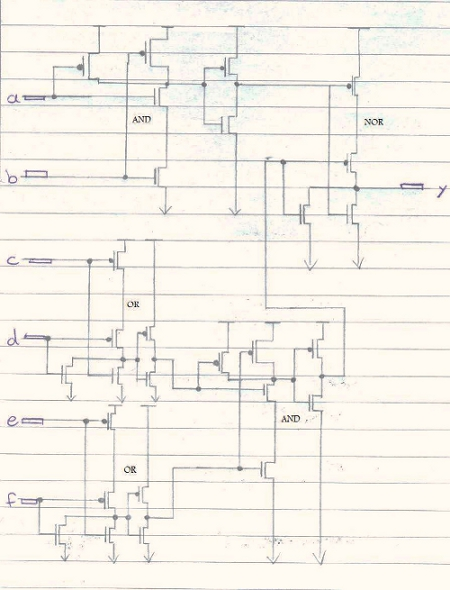
\includegraphics{Schaltskizze93a}

subsection{(b)}
Dieses Komplexgatter benötigt 28 Transistoren, eine herkömmliche CMOS-Gatter-Realisierung dagegen nur 12.


\section{Aufgabe 9.4}
\subsection{(a)}
\subsection{(b)}
\subsection{(c)}
\subsection{(d)}

\section{Aufgabe 9.5}
\subsection{(a)}
\subsection{(b)}

\end{document}
